\chapter{Pokyny pro spuštění přiložených skriptů}

Tato příloha popisuje nastavení prostředí a spuštění přiložených skriptů k reprodukci dosažených výsledků. K provedení experimentů byl využit superpočítač Karolina a konkrétní využité skripty lze nalézt v přiložené složce \verb|karolina/|. Pro ruční spuštění Python skriptů je nezbytné je spouštět ve složce \verb|src/|.

\section{Nastavení prostředí}

Ke spuštění poskytnutých skriptů je třeba nainstalovat potřebné knihovny, připravit použitou datovou sadu, která je podmnožinou datové sady ImageNet, a natrénovat vstupní model neuronové sítě. Tato kapitola provází tímto úvodním nastavením prostředí.  

\subsection{Instalace potřebných knihoven}

K instalaci potřebných knihoven lze využít nástroj Conda a pro něj připraveného prostředí. Prostředí se vytvoří za pomocí příkazu:
\begin{lstlisting}
$ conda create --file environment_linux_x86.yml
\end{lstlisting}

\subsection{Datová sada}

Pro načtení datové sady při běhu systému je použita knihovna TensorFlow Datasets. Přiložený archiv \verb|tiny_imagenet100.tar| s datovou sadou proto musí být rozbalen ve složce \verb|~/tensorflow_datasets/|. Výchozí složku pro datové sady lze v knihovně TensorFlow Datasets předefinovat za pomocí proměnné prostředí \verb|TFDS_DATA_DIR|.

\subsection{Trénování vstupního modelu neuronové sítě}

Poskytnuté soubory obsahují model konvoluční neuronové sítě použitý při experimentech \verb|mobilenet_tinyimagenet_025.keras|. K jeho natrénování byl použit následující příkaz:
\begin{lstlisting}
$ python3 mobilenet_tinyimagenet_train.py \
  --save-as mobilenet_tinyimagenet_0_25.keras \
  --lr 0.025 \
  --batch-size 64 
\end{lstlisting}

\section{Spuštění evolučního algoritmu}

Ke spuštění evolučního algoritmu s poskytnutým modelem neuronové sítě a při použití per-tensor asymetrické kvantizace vah a aproximační metody řešení skládání batch normalizace lze použít následující příkaz:
\begin{lstlisting}
$ python3 run_nsga.py \
  --generations 20 \
  --parent-size 16 \
  --offspring-size 16 \
  --logs-dir <nsga_run_log_dir> \
  --approx
\end{lstlisting}

Po skončení běhu evolučního algoritmu je nutné provést finální evaluaci nejlepších nalezených řešení. K tomu slouží příkaz:
\begin{lstlisting}
$ python3 nsga_evaluate.py --run <nsga_run_log_dir>/<run_file>
\end{lstlisting}

\section{Vizualizace výsledků}

Pro vizualizaci výsledných nalezených řešení slouží skript \verb|show_layer_configuration.py|. Jeho použití je následující:
\begin{lstlisting}
$ python3 show_layer_configuration.py --run <nsga_run_log_dir>
\end{lstlisting}

Následně se zobrazí nabídka k výběru konfigurace k zobrazení. Výsledná vizualizace konfigurace je zobrazena na~obrázku~\ref{fig:appendix_a_show_layer_configuration}.

\begin{figure}[hbt]
	\centering
	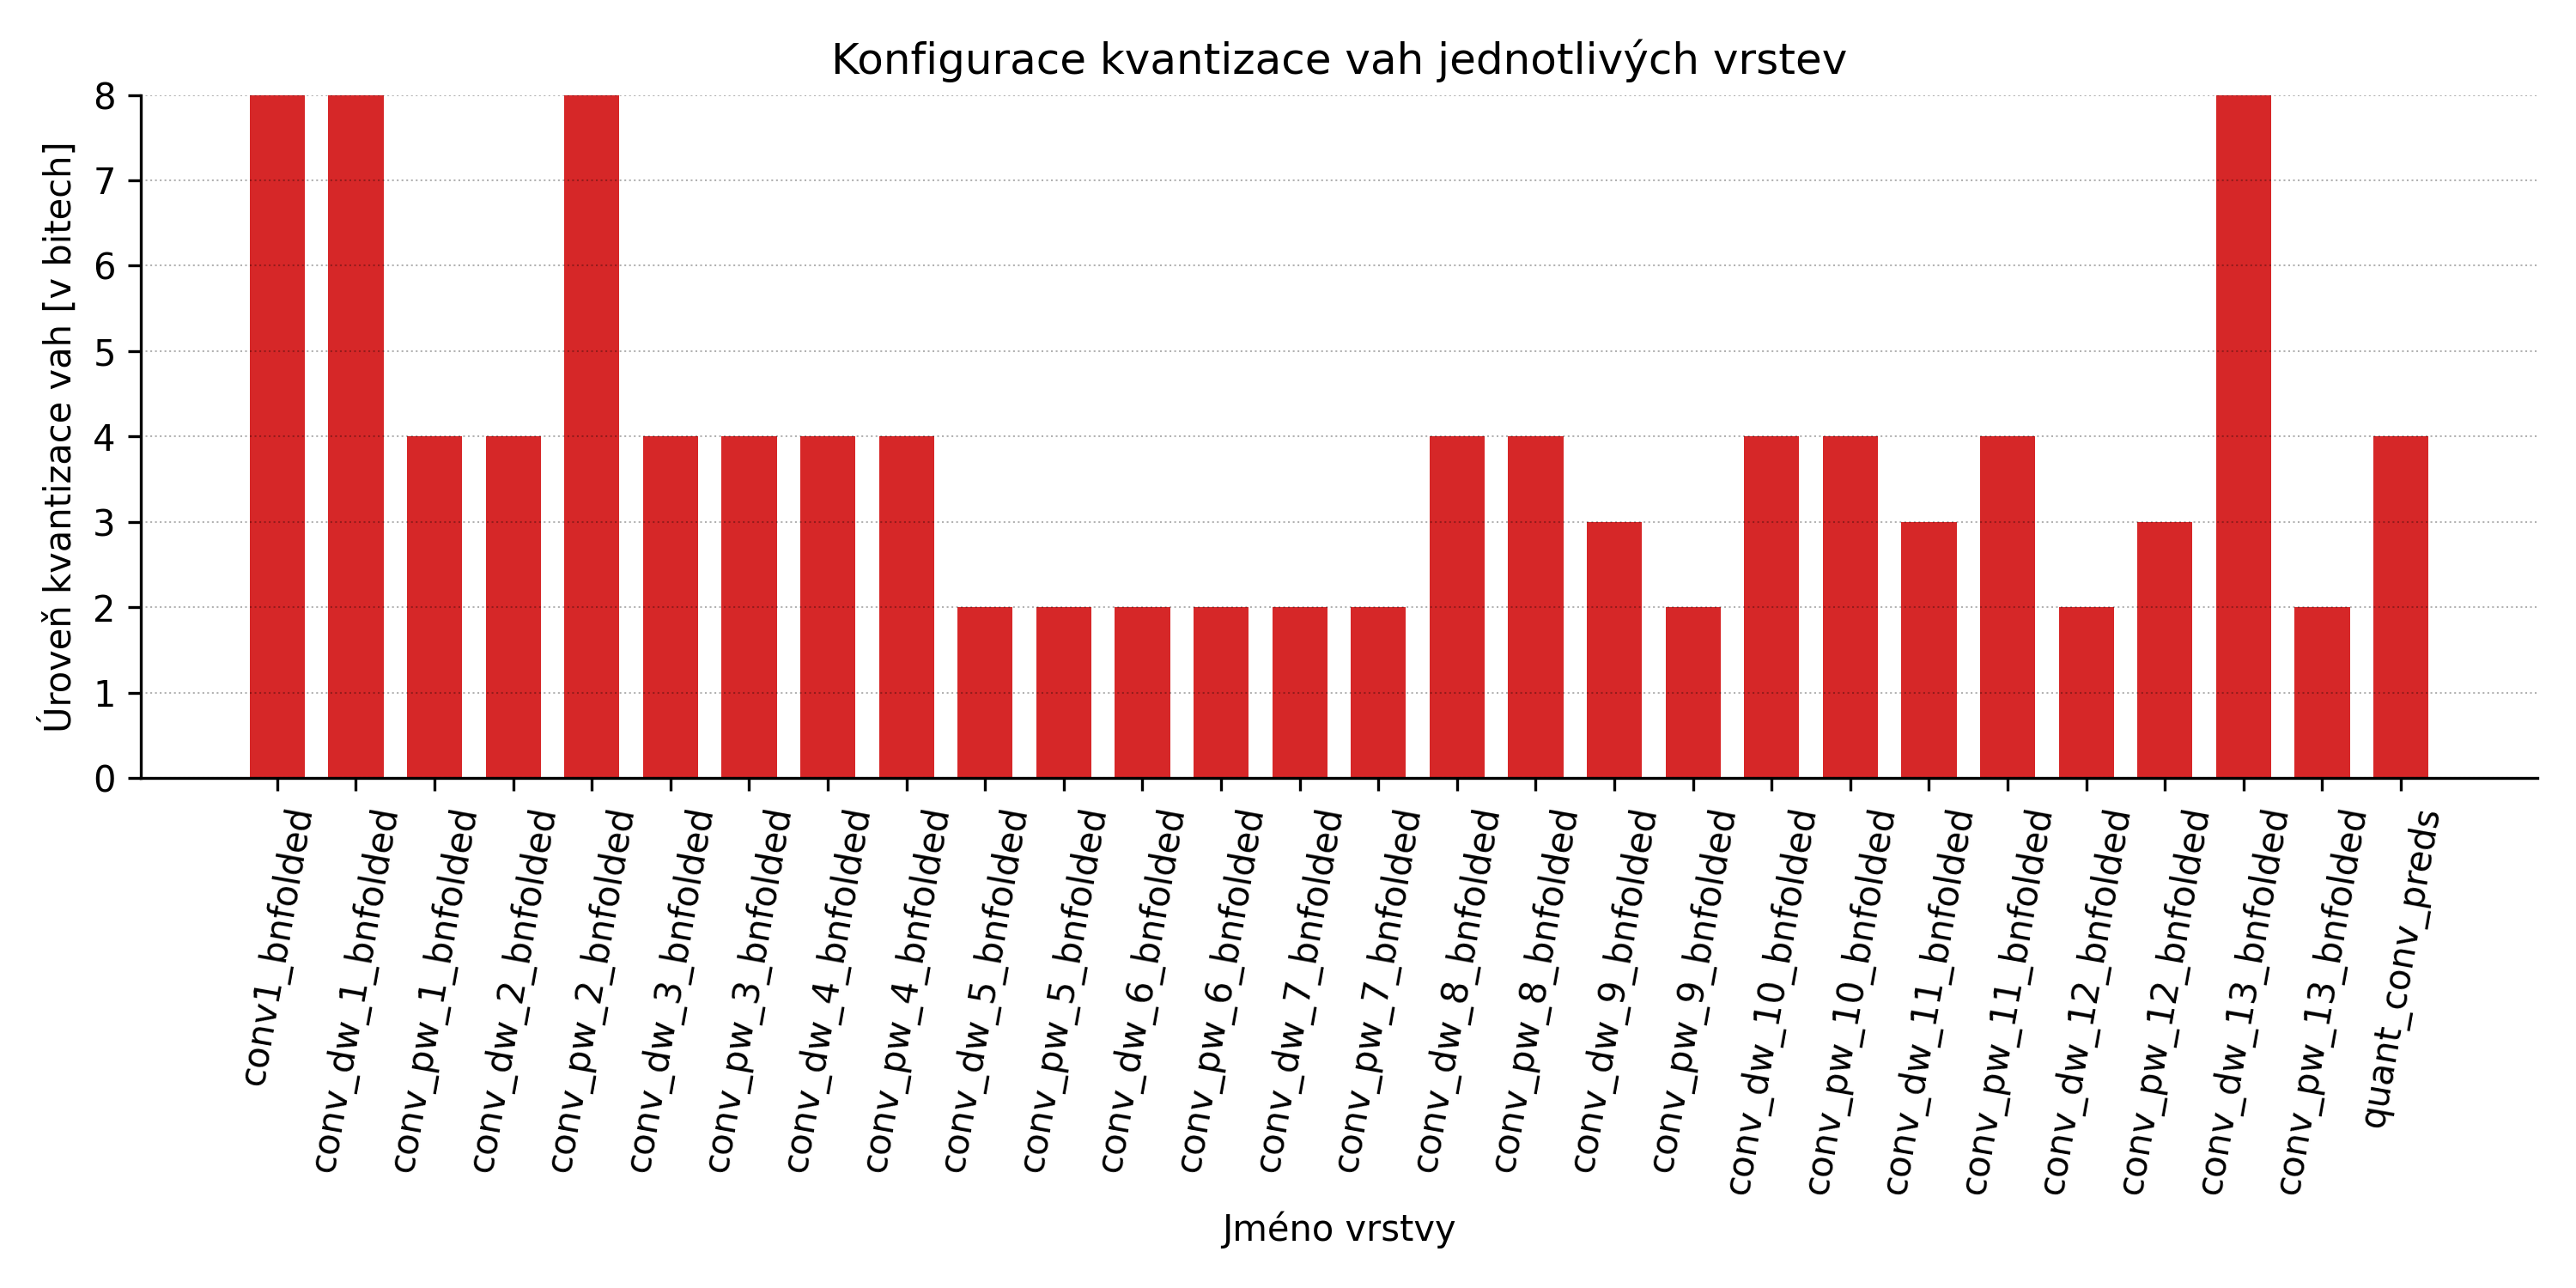
\includegraphics[width=\textwidth]{xsafar23-bp/obrazky-figures/appendix/conf_8_8_4_3_2_8_4_4_4_2_2_2_4_3_4_4_4_4_3_2_8_4_4_2_2_2_4_2_8_True_True.png}
	\caption{Vizualizace nalezené konfigurace kvantizace jednotlivých vrstev pomocí skriptu show\_layer\_configuration.py.}
	\label{fig:appendix_a_show_layer_configuration} 
\end{figure}

\chapter{Obsah přiloženého paměťového média}

\subsection*{Adresářová struktura}

\dirtree{%
 .1 .
 .2 src -- Adresář obsahující zdrojové soubory navrženého systému. 
 .3 tf\_quantization -- Zdrojové soubory k TensorFlow rozšíření. 
 .3 nsga -- Zdrojové soubory implementace NSGA-II algoritmu. 
 .3 datasets -- Zdrojové soubory pro práci s datasetem tiny-imagenet. 
 .3 run\_nsga.py -- Skript sloužící ke spuštění evolučního algoritmu. 
 .3 nsga\_evaluate.py -- Skript určený ke spuštění doladění nalezených řešení.
 .3 show\_layer\_configuration.py -- Skript sloužící k vizualizaci bitové šířky jednotlivých vrstev nalezených řešení. 
 .3 \dots. 
 .2 karolina -- Adresář obsahující scripty použité pro spuštění experimentů. 
 .2 latex -- Adresář obsahující zdrojové soubory pro text práce. 
 .2 README.md -- Návod na použití navrženého systému. 
 .2 nsga\_runs -- Logy běhů evolučního algoritmu pro provedené experimenty. 
 .2 automated\_quantization\_of\_neural\_networks\_paper.pdf -- Text práce. 
  .2 automated\_quantization\_of\_neural\_networks\_paper\_print.pdf -- Text práce pro tisk. 
 .2 environment\_linux\_x86.yml -- Conda prostředí pro operační systém Linux. 
 .2 environment\_macos\_arm64.yml -- Conda prostředí pro Apple Silicon počítače. 
 .2 \dots. 
}